\subsection{Ladeablauf}\label{sec:ladeablauf}

...........Die Betriebszeit des Dojos ermöglicht eine Betriebszeit von fünf Stunden, wobei durch Ladezyklen zwischen den Besuchen eine ganztägiger Betrieb ermöglicht wird. Darum wurde im Ziel 5.1 ein Arbeitstag genannt. Um dies zu veranschaulichen, gibt nachfolgende Abbildung \ref{fig:Ladezyklus Dojo} einen Einblick ins Konzept.

\begin{figure}[H]
	\begin{center}
		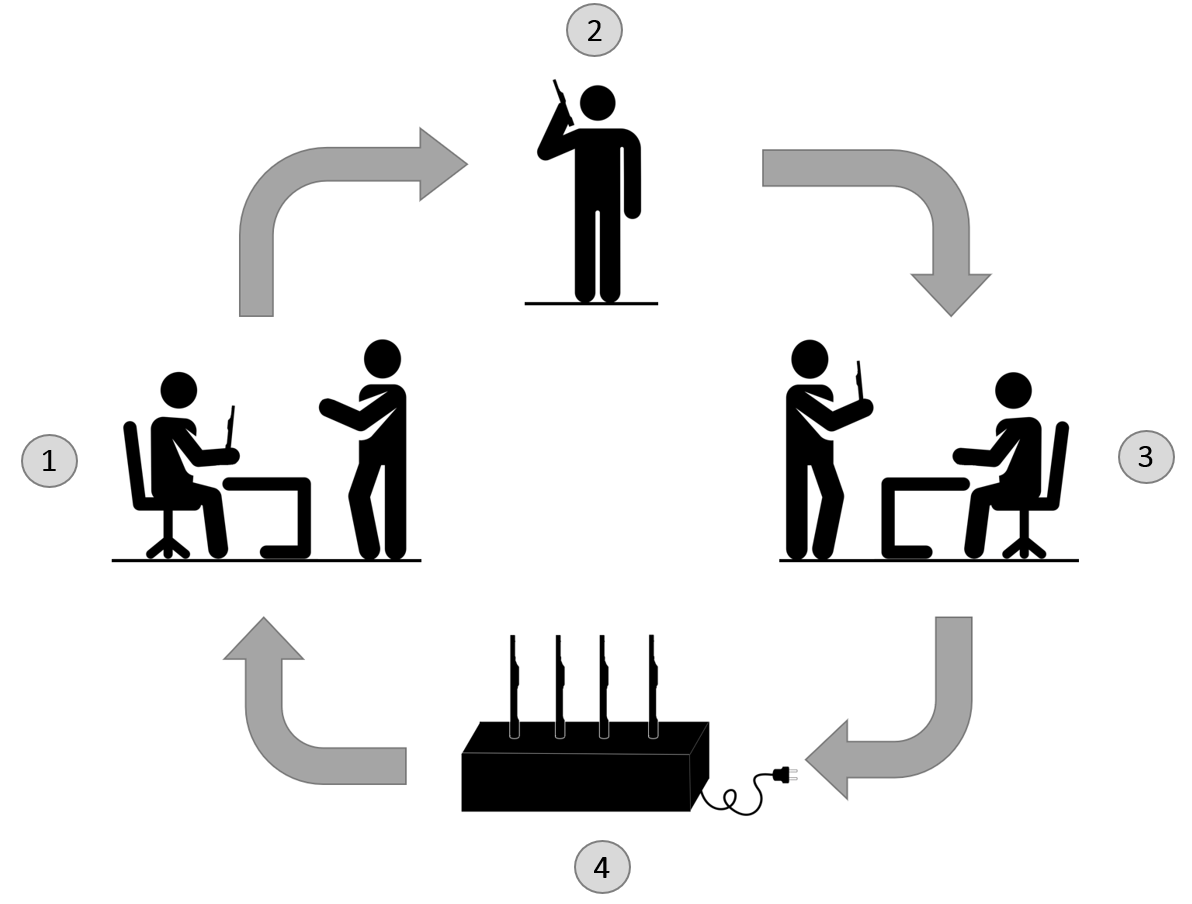
\includegraphics[width=140mm]{data/Ladezyklus2.png}
		\caption[Ladezyklus Dojo]{Ladezyklus Dojo} %picture caption
		\label{fig:Ladezyklus Dojo}
	\end{center}
\end{figure}

Bei Schritt 1 erfolgt die Dojo Ausgabe. Hierbei wird bereits festgelegt welche Sprache verwendet und in welche Bereiche der Besucher Zutritt erhalten soll.
\\
In Schritt 2 befindet sich der Besucher auf dem Rundgang mit dem Dojo als Audio-Guide. Der Nutzer hat die Möglichkeit während dem Rundgang Bilder zu \glqq liken\grqq .
\\
Die Abgabe erfolgt in Schritt 3. Hier kann der Besucher \glqq gelikte\grqq Bilder als Broschüre ausdrucken lassen oder per Mail zusenden lassen.


Wie bereits oben beschrieben, beträgt die Betriebszeit eines durchschnittlichen Rundganges rund drei bis vier Stunden. Sobald die Rückgabe erfolgt ist, wird das Dojo in die Ladebuchse gesteckt wobei immer diese Dojos rausgegeben werden, welche sich am längsten in der Ladestation befinden. Bei einer Stückzahl welche grösser ist als die Besucherzahl, erlaubt dies einen lückenlosen Betrieb.
\cite{Plank}
